%! Author = partsjoo
%! Date = 16.04.2023


Before choosing any options the given set was pre-analyzed using analyze utility to determine the \ac{SA} of the set.
Anonymization options were redefined during the process many times to yeild desired result, but for the baseline settings the first chosen
settings were synthesised quite subjectively. Data set is a sample set of COVID-19 health related data, see Figure~\ref{fig:my_label3}
for example.

\begin{figure}[ht]
  \centering
  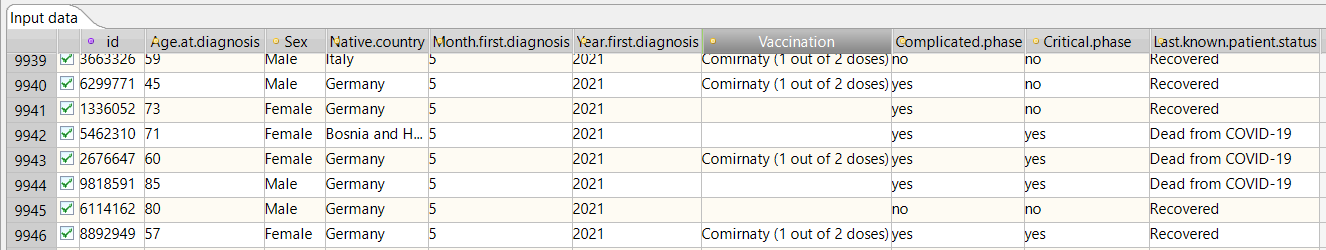
\includegraphics[width=\textwidth, keepaspectratio]{assets/sample_data}
  \caption{Preview of the sample set}
  \label{fig:my_label3}
\end{figure}

\begin{table}[ht]
  \small
  \centering
  \caption{Chosen Generalizations}
  \begin{tabular}{lll}
    \toprule
    \textbf{Generalization}      & \textbf{Levels} & \textbf{Field}            \\
    \midrule
    --                           & Level 1         & id                        \\
    Intervals (5y)               & 6 levels        & Age.at.diagnosis          \\
    Ordering                     & 1 levels        & Sex                       \\
    Priority grouping descending & 3 levels        & Native.country            \\
    --                           & --              & Month.first.diagnosis     \\
    Intervals                    & 2 levels        & Year.first.diagnosis      \\
    Priority grouping            & 3 levels        & Vaccination               \\
    --                           & --              & Complicated.phase         \\
    --                           & --              & Critical.phase            \\
    Priority grouping            & 3 levels        & Last.known.patient.status \\
    \bottomrule
  \end{tabular}\label{tab:table2}
\end{table}


\begin{figure}[ht]
  \centering

  \begin{subfigure}{0.49\textwidth}
    \centering
    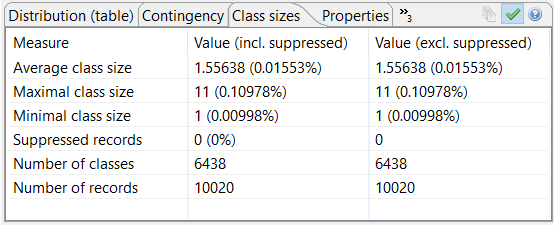
\includegraphics[width=\linewidth]{assets/class_size_unsupressed}
    \caption{Class size unsuppressed}
    \label{fig:subim1}
  \end{subfigure}
  \hfill
  \begin{subfigure}{0.49\textwidth}
    \centering
    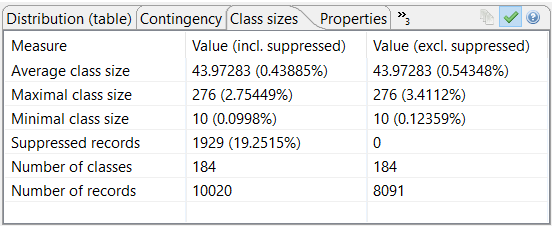
\includegraphics[width=\linewidth]{assets/class_size_supressed}
    \caption{Class size suppressed}
    \label{fig:subim2}
  \end{subfigure}

  \caption{Class size suppressions before and after}
  \label{fig:image2}
\end{figure}
